% !TEX root = ../Build/main.tex
% ###################################################################
% Copyright (c) 2017-2018, Editors: A.D. Rollett & M. De Graef
% All rights reserved.
%
% Licensed under the Creative Commons CC BY-NC-SA 4.0 License, 
% hereafter referred to as the "License"; you may not use this 
% document except in compliance with the License. You may obtain 
% a copy of the License at https://creativecommons.org/licenses/by-nc-sa/4.0/legalcode. 
% Unless required by applicable law or agreed to in writing, all 
% material distributed under the License is distributed on an 
% ``AS IS'' BASIS, WITHOUT WARRANTIES OR CONDITIONS OF ANY KIND, 
% either express or implied. See the License for the specific language 
% governing permissions and limitations under the License.
% ###################################################################

%----------------------------------------------------------------------------------------
%	TITLE PAGE
%----------------------------------------------------------------------------------------

\renewcommand{\chaptergraphicspath}{matter/eps/}

\begingroup
\thispagestyle{empty}
\begin{tikzpicture}[remember picture,overlay]
\coordinate [below=11.4cm] (midpoint) at (current page.north);
\node at (current page.north west)
{\begin{tikzpicture}[remember picture,overlay]
\node[anchor=north west,inner sep=0pt] at (0,0) {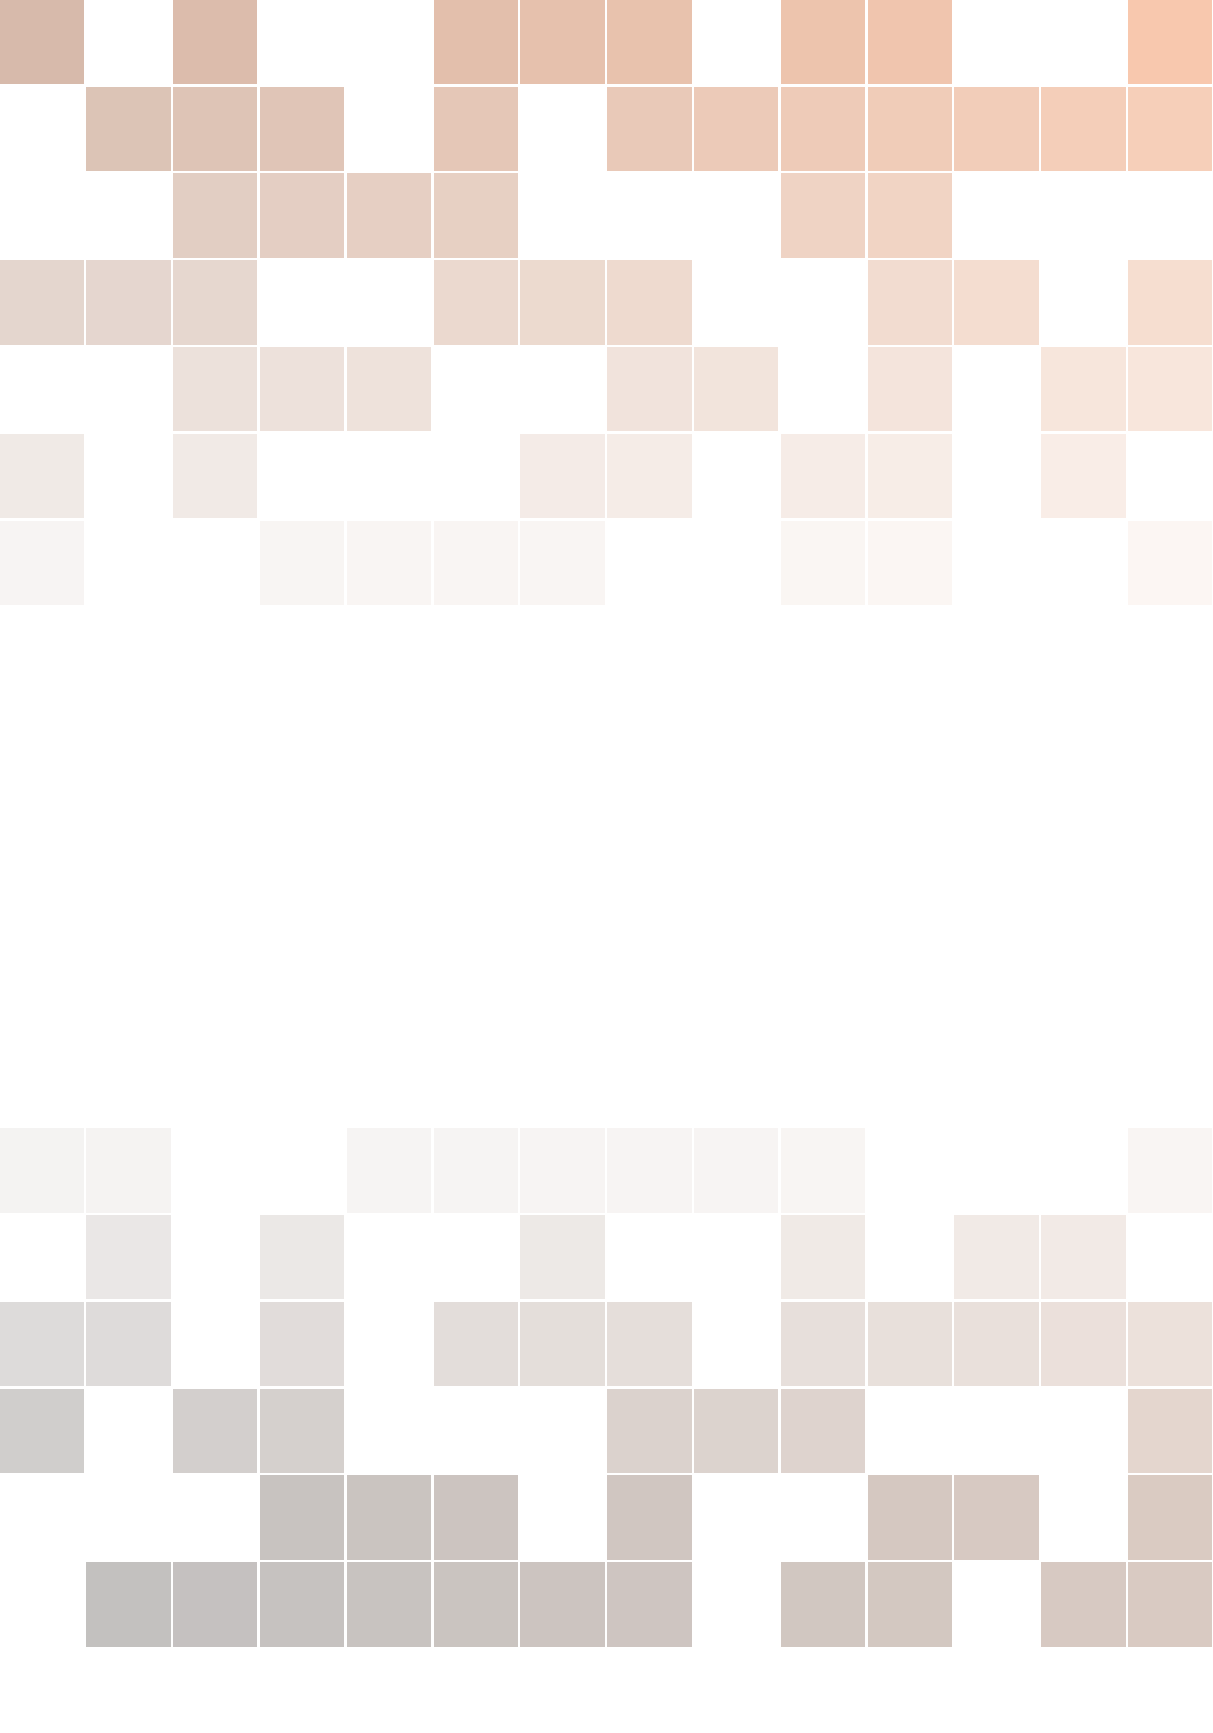
\includegraphics[width=\paperwidth]{../eps/background.pdf}}; % Background image
% the book title may become a user defined variable in a later version
\draw[anchor=north] (midpoint) node [fill=ocre!30!white,fill opacity=0.6,text opacity=1,inner sep=0.6cm]{\Huge\centering\bfseries\sffamily\parbox[c][][t]{\paperwidth}{\centering Microstructure and Properties of Materials\\[10pt] % Book title
% book subtitle
{\Large An Open Source Collection For}\\% Subtitle
{\Large Materials Scientists and Engineers, Physicists, and Geologists}\\[10pt] % Subtitle
% Editor names here
{\huge Editors: Anthony D. Rollett and Marc De Graef}\\[10pt] {\Large Department of Materials Science and Engineering\\[-10pt] Carnegie Mellon University}}};
\end{tikzpicture}};
\end{tikzpicture}
\vfill
\endgroup

%----------------------------------------------------------------------------------------
%	COPYRIGHT PAGE
%----------------------------------------------------------------------------------------

\newpage
~\vfill
\thispagestyle{empty}

\noindent Copyright \copyright\ 2017-2025\\ % Copyright notice

\noindent \textsc{Published by the Department of Materials Science and Engineering, Carnegie Mellon University}\\ % Publisher

\noindent \textsc{Partially funded by the National Science Foundation, grant No.\ DMR-1904629.}\\ 

%\noindent \textsc{OpenChapters.web.cmu.edu}\\ % URL

\noindent Licensed under the Creative Commons CC BY-NC-SA 4.0 License, hereafter referred to as the ``License''); you may not
use this document except in compliance with the License. You may obtain a copy
of the License at \url{https://creativecommons.org/licenses/by-nc-sa/4.0/legalcode}. Unless
required by applicable law or agreed to in writing, all material distributed
under the License is distributed on an ``AS IS'' BASIS, WITHOUT
WARRANTIES OR CONDITIONS OF ANY KIND, either express or implied. See the
License for the specific language governing permissions and limitations
under the License.\index{license}\\ % License information

\noindent \textit{First edition, September 2020}\\ % Printing/edition date
\noindent \textit{Current edition, \monthyear}

\clearpage
%----------------------------------------------------------------------------------------
%	LIST OF CONTRIBUTING AUTHORS
%----------------------------------------------------------------------------------------
\processauthors

\clearpage
%----------------------------------------------------------------------------------------
%	TABLE OF CONTENTS
%----------------------------------------------------------------------------------------

\pagestyle{empty} % No headers
\makeatletter
\begin{tikzpicture}[remember picture,overlay]
\node at (current page.north west)
{\begin{tikzpicture}[remember picture,overlay]
\node[anchor=north west,inner sep=0pt] at (0,0) {\includegraphics[width=\paperwidth]{../eps/TOCheader.pdf}};
\draw[anchor=west] (\Gm@lmargin,-9cm) node [line width=2pt,rounded corners=15pt,draw=ocre,fill=white,fill opacity=0.5,inner sep=15pt]{\strut\makebox[22cm]{}};
\draw[anchor=west] (\Gm@lmargin+.3cm,-9cm) node {\huge\sffamily\bfseries\color{black}Table of Contents\strut};
\end{tikzpicture}};
\end{tikzpicture}
\par\vspace*{150\p@}
\makeatother
\renewcommand{\contentsname}{}
\tableofcontents % Print the table of contents itself
\cleardoublepage % Forces the first chapter to start on an odd page so it's on the right
\pagestyle{fancy} % Print headers again

% not sure if we need this in the front or back matter...
%%\listoffigures
%
%%\listoftables
%
%% dedication
%\cleardoublepage
%~\vfill
%\begin{doublespace}
%\noindent\fontsize{18}{22}\selectfont\itshape
%\nohyphenation
%Dedicated to $\ldots$.
%\end{doublespace}
%\vfill
%\vfill


%
%\cleardoublepage
%\chapterimage{chapter_head_2.pdf} % Chapter heading image
%
%\chapter*{Preface}
%
%% the following sections should really come from user-defined text (except for the last one) since this
%% will be different for each custom text book...
% 
%\section*{Who should read this book?}
%
%
%
%\section*{What is in this book?}
%We begin this book with rotations in 2D; this will serve as a review as well as an opportunity to define several important concepts, including \textit{active} and \textit{passive} rotations, \textit{positive} and \textit{negative} rotation angles, and so on.  Then we cover 3D rotations in section~\ref{sec:3Drotations} using only rotation matrices; we will introduce the concept of a special orthonormal matrix and the related space of 3D orientations, $SO(3)$.  Euler angles form the topic of section~\ref{sec:eulerangles}; we will introduce the Bunge convention in detail, and also discuss other conventions.  Neo-Eulerian representations are introduced in section~\ref{sec:neoEulerian}; they include the \textit{axis-angle pair}, the \textit{quaternion}, the \textit{Rodrigues-Frank vector}, the \textit{homochoric vector}, and the \textit{stereographic vector}.  Section~\ref{sec:cubochoric} is devoted to the recently introduced \textit{cubochoric} representation.
%
%
%
%The text is heavily illustrated and makes use of numerous examples and exercises.  
%
%
%
%
%
%\section*{What does Open Source mean for this book?}
%This is an \textit{open source}\index{open source} book, meaning that, in addition to this PDF file, we make all the original \LaTeX\ source files and original illustrations available on-line via the GitHub repository.  The copyright for this book falls under the \textit{Creative Commons Attribution-NonCommercial-ShareAlike 4.0 International Public License}\index{license} or CC BY-NC-SA 4.0 for short.  If you are just a reader interested in the material covered in this book, then you do not need to think about this copyright license at all.  If you are a researcher who wishes to use some of the illustrations for your own publications, or if you are an instructor who would like to make printed copies of this text available to a group of students, or if you wish to contribute to this text, then we encourage you to read the detailed license available from \url{https://creativecommons.org/licenses/by-nc-sa/4.0/legalcode}. 
%
%Here is what it means in practice (text taken from the Creative Commons web site): 
%{\small\begin{itemize}
%	\item \textit{\textbf{Sharing:}} you are free to copy and redistribute this material in any medium or format;
%	\item \textit{\textbf{Adapting:}} you are free to remix, transform, and build upon this material. 
%\end{itemize}}
%\noindent You have these freedoms as long as you follow the license terms:
%{\small\begin{itemize}
%	\item \textit{\textbf{Attribution:}}  you must give appropriate credit, provide a link to the license, and indicate if changes were made. You may do so in any reasonable manner, but not in any way that suggests the licensor endorses you or your use;
%	\item \textit{\textbf{NonCommercial:}} you may not use the material for any commercial purposes;
%	\item \textit{\textbf{ShareAlike:}} if you remix, transform, or build upon the material, you must distribute your contributions under the same license as the original.
%\end{itemize}}
%You may not apply legal terms or technological measures that legally restrict others from doing anything the license permits.
%




